\documentclass{article}
\usepackage{indentfirst}
\usepackage[utf8]{inputenc}
\usepackage[T1]{fontenc}
\usepackage[brazilian]{babel}
\usepackage{lmodern}
\usepackage{graphicx}
\usepackage{float}
\usepackage[]{subfigure}
\usepackage{afterpage}
\usepackage{amsmath}
\usepackage{textcomp,gensymb}
\usepackage{nameref}
\usepackage{accents}
\usepackage{listings}
\usepackage{color,soul}
\usepackage[margin=1in]{geometry}
\usepackage{steinmetz}
\usepackage{xfrac}

\PassOptionsToPackage{hyphens}{url}\usepackage{hyperref}
\hypersetup{
    breaklinks = true,
}
\urlstyle{same}
\newcommand{\ubar}[1]{\underaccent{\bar}{#1}}
%\renewcommand\thesection{\arabic{section}$^a$}
\renewcommand\thesection{\arabic{section}.}
\renewcommand\thesubsection{\arabic{section}.\alph{subsection}}
\definecolor{dkgreen}{rgb}{0,0.6,0}
\definecolor{gray}{rgb}{0.5,0.5,0.5}
\definecolor{mauve}{rgb}{0.58,0,0.82}
\lstset{
    frame=tb,
    language=Matlab,
    aboveskip=3mm,
    belowskip=3mm,
    showstringspaces=false,
    basicstyle={\small\ttfamily},
    numbers=none,
    numberstyle=\tiny\color{gray},
    keywordstyle=\color{blue},
    commentstyle=\color{dkgreen},
    stringstyle=\color{mauve},
    breaklines=true,
    breakatwhitespace=true,
    tabsize=4
}

\title{Simulação 4 - Controle Digital}
\author{Arthur de Matos Beggs - 12/0111098}
\date{2021}

\begin{document}
% capa
\begin{titlepage}
    \begin{center}
        \centering
        
\includegraphics[width=.7\linewidth]{images/logo_unb.png}\\[0.5cm]
        {\large \textbf{Universidade de Brasília}}\\[0.2cm]
        {\large \textbf{Departamento de Engenharia Elétrica}}\\[0.2cm]
        {\large \textbf{Controle Digital}}\\[4.8cm]
        {\bf \huge {Exercício de Simulação 4}}\\[0.2cm]
        {\bf \large {}}
    \end{center}

    \vspace{5cm}
    \hspace{2cm} {\noindent \bf \large {Aluno:}}\\
    \vspace{0.8cm}
    \hspace{2.35cm} {\large Arthur de Matos Beggs --------------------------------- 12/0111098}\\[1cm]

    \begin{center}
        {\large Brasília}\\
        {\large 2$^{\ubar{\circ}}$/2020}
    \end{center}

\end{titlepage}

\clearpage % Quebra de página

\setcounter{page}{2}

    \begin{figure}[H]
       \centering
            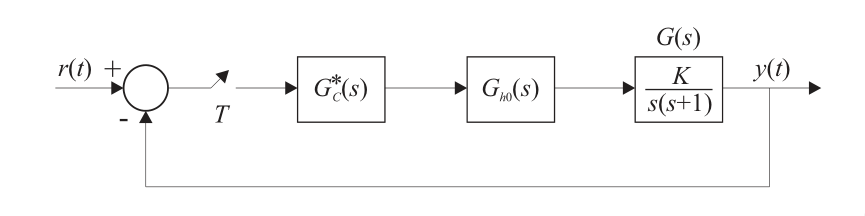
\includegraphics[width=1\linewidth]{images/diagrama.png}
            \caption{Diagrama e funções de transferência do sistema.}
            \label{fig:diagram}
    \end{figure}

\section{\normalsize{Determine a função de transferência $G(z)$ da planta $G(s)$ em série com o segurador de ordem zero $G_{h0}(s)$ e obtenha $G(\omega) = G(z)|_{z = \frac{1 + (\sfrac{T}{2})\omega}{1 - (\sfrac{T}{2})\omega}}$}}

    $$ G(z) = \mathcal{Z}\left\{\frac{ 1 - \mathrm{e}^{-0.2s} }{s} \frac{K}{s(s+1)} \right\}
            = (1-z^-1) \mathcal{Z}\left\{ \frac{K}{s^{2} (s+1)}  \right\} $$\\
    {Pelo Matlab,}
\begin{lstlisting}
T = 0.2;

s = tf('s');
z = tf('z', T);

G_s = zpk([], [0 -1], [1])
G_z = c2d(G_s, T, 'zoh')
\end{lstlisting}
    $$ G(z) = \frac{ 0.018731K(z+0.9355) }{ (z-1)(z-0.8187) } $$
    $$ G(\omega) = G(z)|_{z = \frac{1 + (\sfrac{T}{2})\omega}{1 - (\sfrac{T}{2})\omega}} = G(z)|_{z = \frac{1 + 0.1\omega}{1 - 0.1\omega}} $$

    {Pelo Matlab,}
\begin{lstlisting}
G_w = zpk(tf(bilin(ss(G_z), -1, 'S_Tust', [T 1])))
\end{lstlisting}

    $$ G(\omega) = \frac{-0.00033201K(\omega + 300.2)(\omega -10)}{\omega(\omega + 0.9967)} $$\\


\section{\normalsize{Calcule o valor do ganho $K$ da planta de modo que a constante de erro de velocidade seja $K_v = 2$}}
    {Para que $K_v = 2$,}
    $$ K_v = \lim\limits_{\omega \to 0} \omega G_c(\omega)G(\omega)
           = \lim\limits_{\omega \to 0} \frac{-0.00033201K(\omega + 300.2)(\omega -10)}{(\omega + 0.9967)} G_c(\omega)
           = K \lim\limits_{\omega \to 0} G_c(\omega) $$\\

    {Considerando $G_c(\omega) = 1$ nessa análise,}
    $$ K = K_v = 2 $$


\section{\normalsize{Obtenha o diagrama de Bode para $G(\omega)$}}
    \begin{figure}[H]
       \centering
            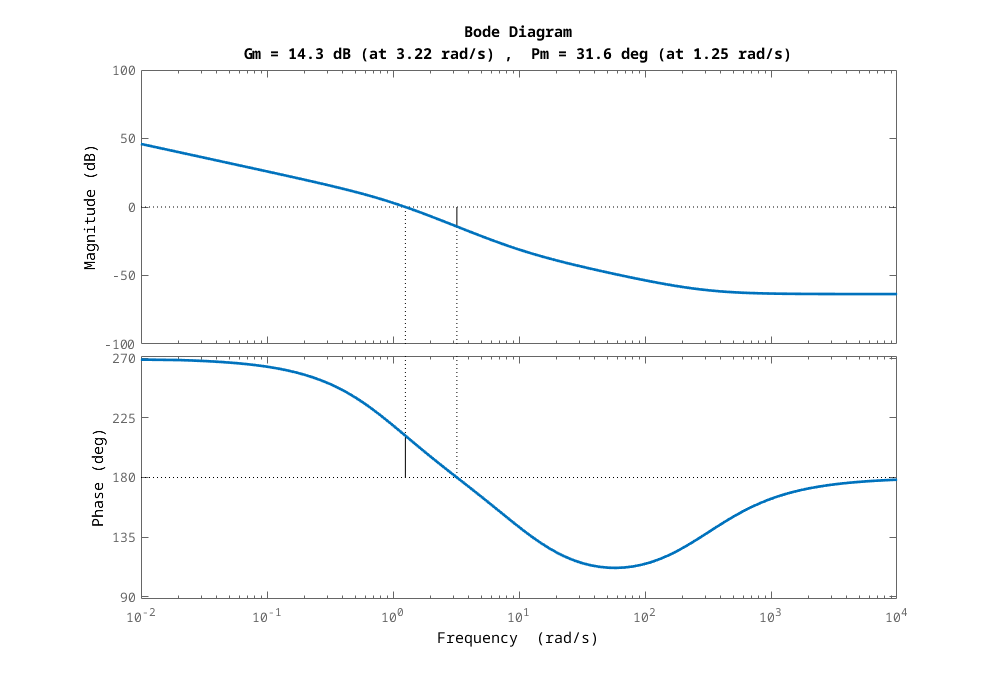
\includegraphics[width=1\linewidth]{images/bode_KG_w.png}
            \caption{Diagrama de Bode de $ G(s) = G(\omega)|_{\omega=s} $}
            \label{fig:bodeG}
    \end{figure}


\section{\normalsize{Calcule o polo e o zero de um compensador por avanço de fase de modo que a margem de fase seja de $50^{\circ}$ e a margem de ganho seja de pelo menos $10 dB$}}
    {O compensador por avanço de fase tem a forma}
    $$ G_c(\omega) = \frac{1 + \tau\omega}{1 + \alpha\tau\omega} $$

    {A Margem de Fase de $G (\omega) $ é de $ 31.6 ^{\circ} $. Para que a Margem de Fase satisfaça o requerimento de $ 50 ^{\circ} $, um avanço de fase de $ \approx 20 ^{\circ} $ é necessário. Porém, também é necessário compensar o deslocamento da frequência de cruzamento. Assim, $ 8 ^{\circ} $ adicionais compensam a frequência de cruzamento, resultando em $ \phi_m = 28 ^{\circ} $. Com isso,}

    $$ \sin(\phi_m) = \frac{ 1-\alpha }{ 1+\alpha } \implies \alpha = 0.361. $$

    {O avanço de fase máximo $\phi_m$ de $G_c(j\nu)$ ocorre em $\nu_m = \frac{1}{\tau \sqrt{\alpha}}$. Em $\nu_m$, $|G_c(j\nu_m)G(j\nu_m)| = 1$. Assim,}
    $$ |G_c(j\nu_m)| = \frac{1}{\sqrt{\alpha}} = 1.644 $$
    $$ |G(j\nu_m)| = \frac{1}{|G_c(j\nu_m)|} = \sqrt{\alpha} = 0.601 \implies \nu_m = 1.2773 $$
    {$\nu_m$ encontrado pelas raízes de $abs((-0.000664 s^2 - 0.1927 s + 1.993)/(s^2 + 0.9967 s)) = 0.601$ no WolframAlpha.}

    {Assim,}
    $$ \nu_m = \frac{1}{\tau \sqrt{\alpha}} \implies \tau = 1.3027 $$
    $$ G_c(\omega) = \frac{1 + \tau\omega}{1 + \alpha\tau\omega} = \frac{1 + 1.3027\omega}{1 + 0.4703\omega} $$

    {Para encontrar $G_c(z)$, a transformação bilinear $G_c(z) = G_c(\omega)|_{\omega = \frac{2}{T}\frac{z-1}{z+1}}$ pelo Matlab,}
\begin{lstlisting}
Gc_w = tf([1.3027 1], [0.4703 1])
Gc_z = zpk(tf(bilin(ss(Gc_w), 1, 'S_Tust', [T 1])))
\end{lstlisting}
    $$ G_c(z) = G_c(\omega)|_{\omega = \frac{2}{T}\frac{z-1}{z+1}} = \frac{2.4596(z-0.8574)}{(z-0.6493)} $$


\section{\normalsize{Faça os diagramas de Bode de $G(\omega)$, $G_c(\omega)$ e $G_c(\omega)G(\omega)$}}
    \begin{figure}[H]
       \centering
            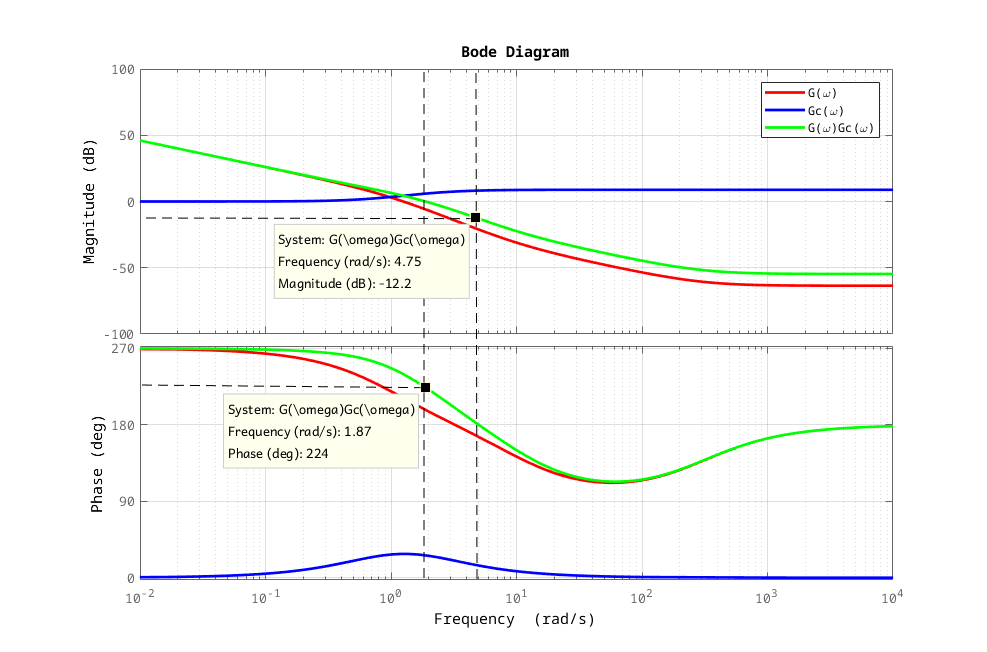
\includegraphics[width=1\linewidth]{images/bode_omega.png}
            \caption{Diagrama de Bode de $G(\omega)$, $G_c(\omega)$ e $G_c(\omega)G(\omega)$}
            \label{fig:bode_omega}
    \end{figure}

    {Pelo diagrama, a margem de fase de $G_c(\omega)G(\omega) \approx 44^\circ$ e a margem de ganho de $G_c(\omega)G(\omega) \approx 12.2 dB$. A margem de ganho segue as especificações do projeto ($> 10 dB$), mas a margem de fase ficou $6^\circ$ abaixo do requisito.}


\section{\normalsize{Faça os diagramas de Bode de $G(z)$, $G_c(z)$ e $G_c(z)G(z)$ para $z = e^{j\omega T}$}}
    \begin{figure}[H]
       \centering
            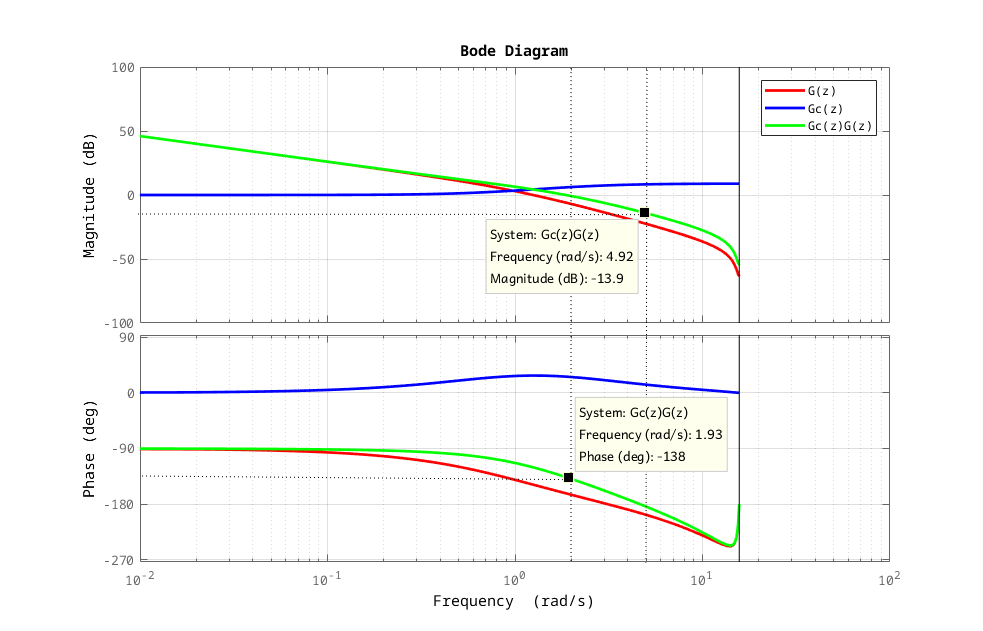
\includegraphics[width=1\linewidth]{images/bode_z.png}
            \caption{Diagrama de Bode de $G(z)$, $G_c(z)$ e $G_c(z)G(z)$}
            \label{fig:bode_z}
    \end{figure}

    {Utilizando o comando $margin()$ para obter valores mais precisos de margem de ganho e de fase que os mostrados pelo cursor no diagrama de Bode da Figura~\ref{fig:bode_z}, a margem de fase de $G_c(z)G(z) \approx 44^\circ$ e a margem de ganho de $G_c(z)G(z) \approx 12.9 dB$. A margem de ganho segue as especificações do projeto ($> 10 dB$), mas a margem de fase ficou $6^\circ$ abaixo do requisito.}

    {Os resultados das margens de fase e de ganho do sistema tanto em $z$ quanto em $\omega$ são bem próximos.}



\end{document}
